\section{Results}
\label{sec:results}

We present results in causal chain order: existence $\to$ selection signal $\to$ training gradient concentration.

\subsection{RQ1: Variance Distribution (h-e1) --- PASSED}

\textbf{The distribution is severely right-skewed, but a meaningful high-variance subset exists.}

\begin{table}[h]
\centering
\caption{MBPP pass rate distribution (374 problems, $k=4$, \texttt{max\_new\_tokens=128}).}
\label{tab:distribution}
\begin{tabular}{lrrl}
\toprule
Pass Rate ($p_i$) & Count & Percentage & Variance ($v_i$) \\
\midrule
0.00 (all-fail) & 343 & 91.7\% & 0.0000 \\
0.25 (1/4 pass) & 29 & 7.8\% & \textbf{0.1875} \\
0.50 (2/4 pass) & 0 & 0.0\% & 0.2500 \\
1.00 (all-pass) & 2 & 0.5\% & 0.0000 \\
\bottomrule
\end{tabular}
\end{table}

29 problems satisfy $v_i > 0.1$, exceeding the gate threshold of 15 (PASSED). The 91.7\% per-problem all-fail rate under profiling ($k=4$, \texttt{max\_new\_tokens=128}) substantially exceeds Nie et al.'s 54.75\% all-fail component, suggesting that constrained generation parameters may amplify practical gradient starvation beyond theoretical estimates for this model.

\begin{figure}[t]
\centering
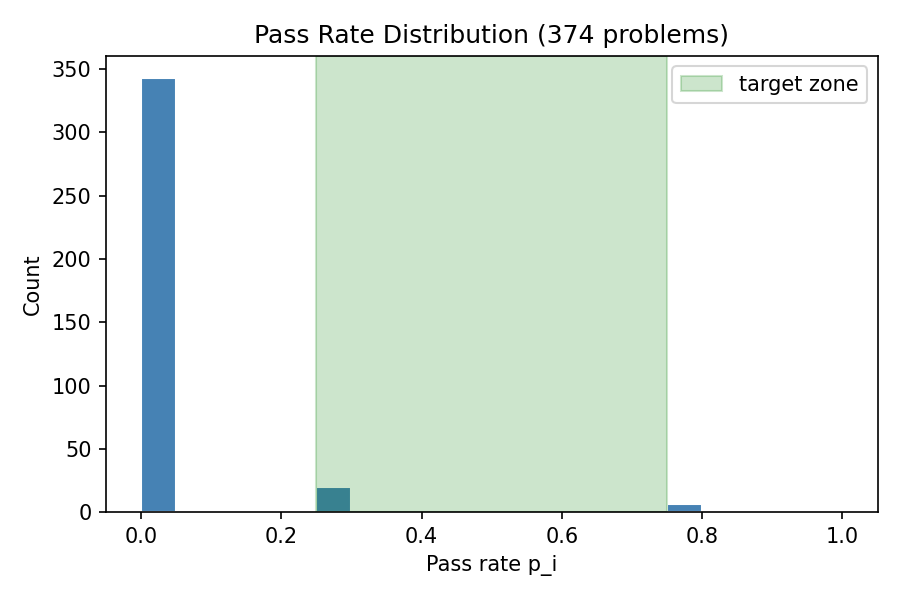
\includegraphics[width=0.9\textwidth]{figures/fig2_pass_rate_histogram.png}
\caption{Pass rate histogram for 374 MBPP problems under constrained generation ($k=4$, \texttt{max\_new\_tokens=128}). The distribution is bimodal: a dominant mass at $p_i=0$ (343 problems, 91.7\%) and a small spike at $p_i=0.25$ (29 problems, 7.8\%). No problems achieve $p_i=0.5$ under these generation constraints.}
\label{fig:pass_rate_hist}
\end{figure}

\begin{figure}[t]
\centering
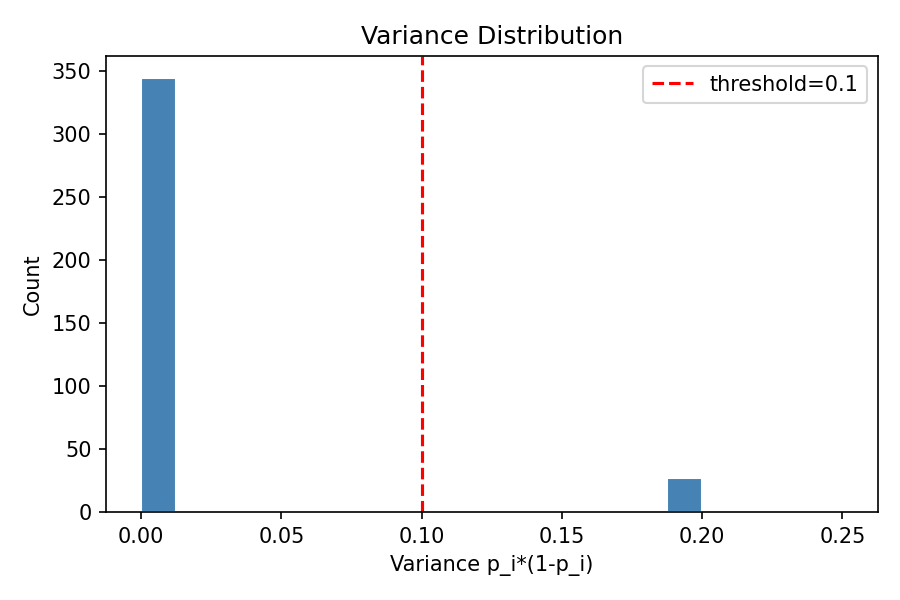
\includegraphics[width=0.9\textwidth]{figures/fig3_variance_histogram.png}
\caption{Binary execution reward variance distribution across 374 MBPP problems. 343 problems have $v_i=0$ (all-fail or all-pass); 29 have $v_i=0.1875$ (the maximum achievable under $k=4$ discrete sampling). No intermediate variance levels exist under these generation constraints.}
\label{fig:variance_hist}
\end{figure}

\textbf{Gate verdict (h-e1): PASSED} --- existence of gradient-signal subset confirmed.

\subsection{RQ2: Selection Signal (h-m1) --- PASSED}

\textbf{Variance-guided selection achieves $4.24\times$ higher mean variance than random selection ($p=2.22\times10^{-6}$).}

\begin{table}[h]
\centering
\caption{Variance selection comparison: top-50 variance-guided vs.\ random-50.}
\label{tab:selection}
\begin{tabular}{lllll}
\toprule
Metric & Variance-50 & Random-50 & Difference & $p$-value \\
\midrule
Mean variance & \textbf{0.1113} & 0.0262 & 0.0850 & $2.22\times10^{-6}$ \\
Ratio & \textbf{$4.24\times$} & $1.0\times$ & --- & --- \\
Mann-Whitney U & 1807.0 & --- & --- & $2.22\times10^{-6}$ \\
\bottomrule
\end{tabular}
\end{table}

\begin{figure}[t]
\centering
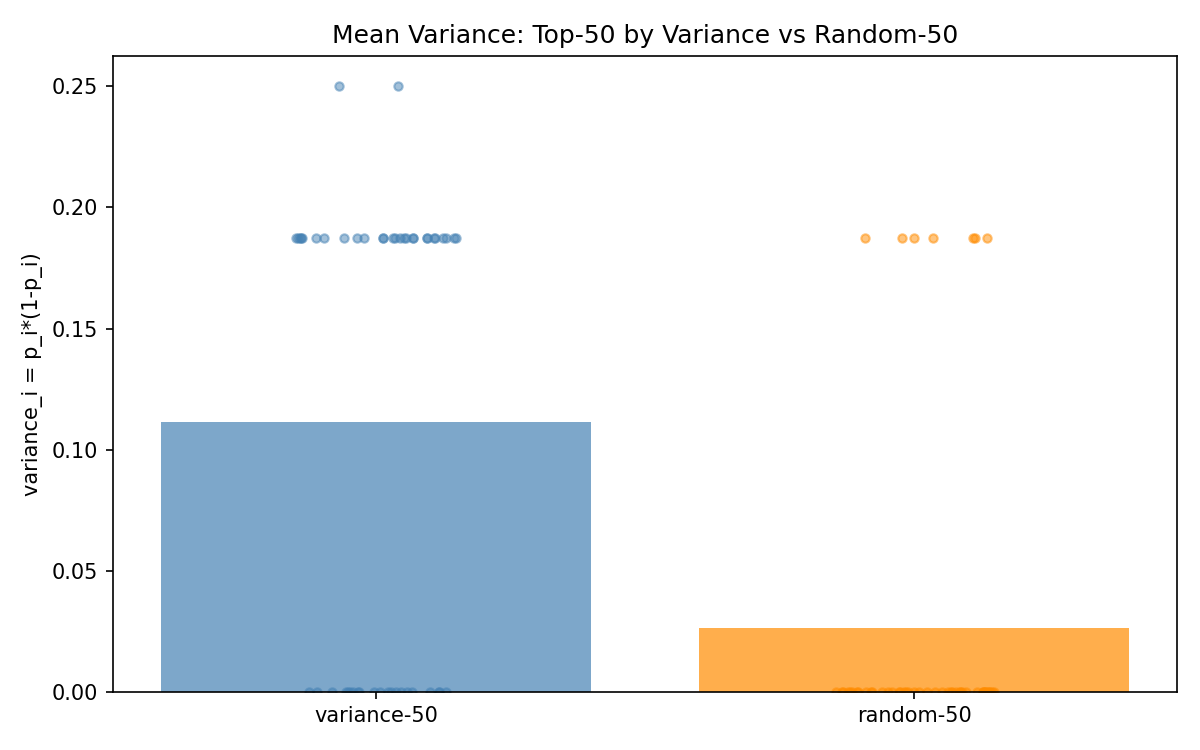
\includegraphics[width=0.9\textwidth]{figures/fig1_mean_comparison.png}
\caption{Mean variance comparison between variance-guided top-50 selection and random-50 selection, with individual data points overlaid. Variance-guided selection achieves $4.24\times$ higher mean variance (Mann-Whitney $p=2.22\times10^{-6}$), confirming a statistically robust selection signal.}
\label{fig:mean_comparison}
\end{figure}

\begin{figure}[t]
\centering
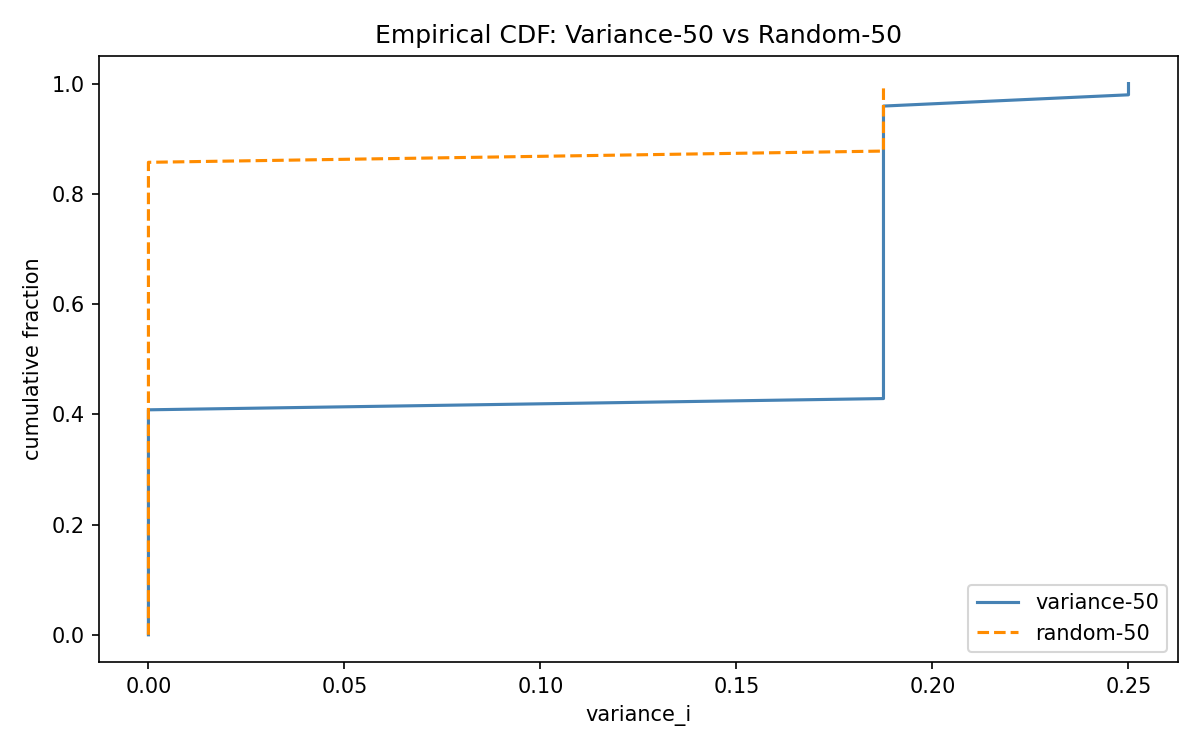
\includegraphics[width=0.9\textwidth]{figures/fig4_cdf.png}
\caption{Empirical CDFs of per-problem variance for variance-50 and random-50 selections. The variance-guided CDF lies entirely to the right of the random-50 CDF, confirming stochastic dominance: variance-guided selection produces higher variance at every quantile.}
\label{fig:cdf}
\end{figure}

The selection signal is not marginal. Even with 21 zero-variance filler problems in the variance-50 set (\texttt{boundary\_gap=0}, all 29 high-variance problems in the top-50), the overall distribution dramatically differs from random selection.

\textbf{Gate verdict (h-m1): PASSED} --- selection signal confirmed.

\subsection{RQ3: Gradient Concentration During Training (h-m2, h-m3) --- FAILED}

\textbf{Both conditions show \texttt{frac\_reward\_zero\_std=1.0} throughout all training steps --- cold-start confirmed.}

\textbf{h-m2 (50 steps, LR=$5\times10^{-7}$):} Both variance-50 and random-50 maintained \texttt{frac\_reward\_zero\_std=1.0} at every step. \texttt{reward/mean=0.0}, \texttt{grad\_norm=0.0} throughout. Total generation attempts: $50 \text{ steps} \times 50 \text{ problems} \times 4 \text{ completions} = 10{,}000$, all returning reward=0.

\textbf{h-m3 (200 steps, LR=$1\times10^{-6}$):} Cold-start persisted despite doubled learning rate and $4\times$ more training steps. \texttt{frac\_reward\_zero\_std=1.0} throughout 200 steps. Additional 40,000+ generation attempts, all reward=0.

\textbf{Combined: 50,000+ generation attempts, zero reward across all conditions.}

\begin{figure}[t]
\centering
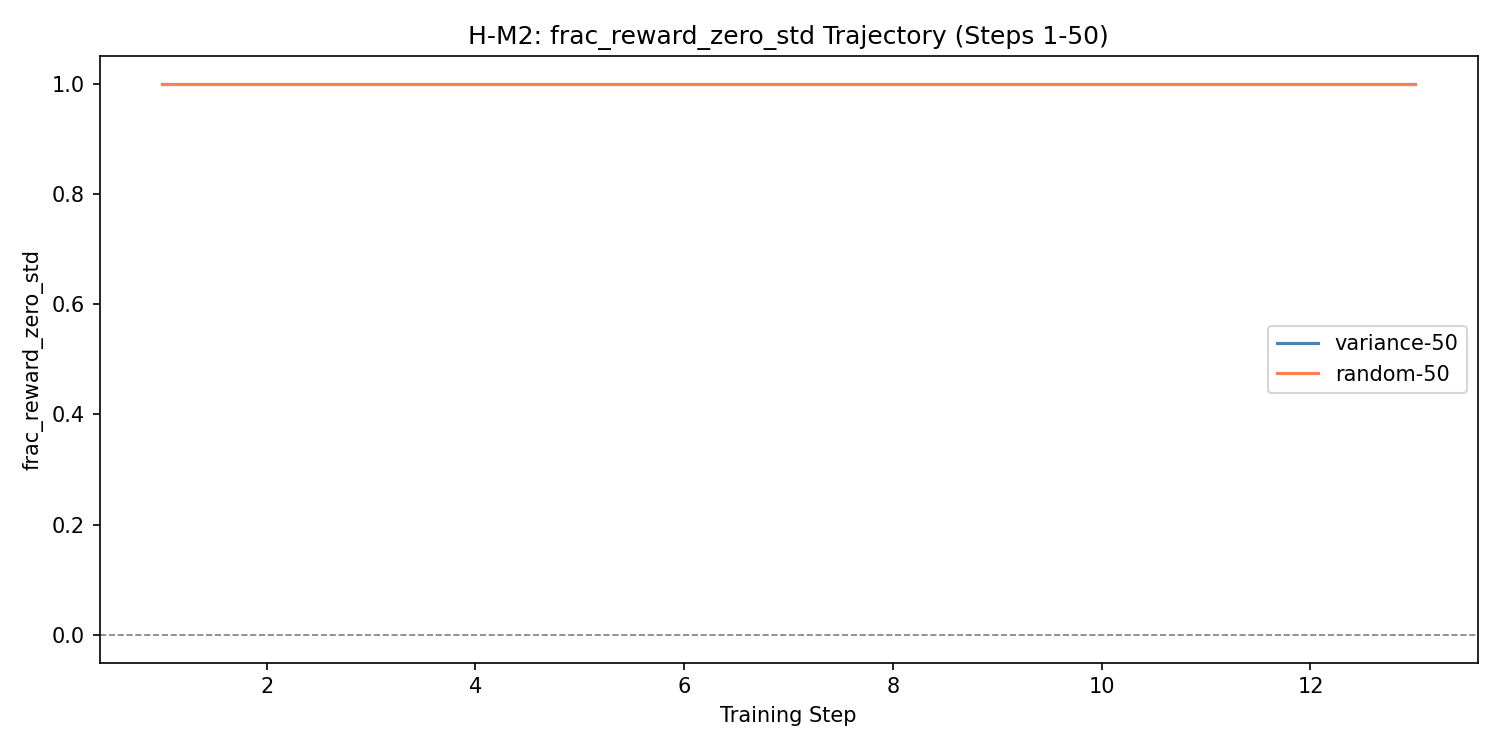
\includegraphics[width=0.9\textwidth]{figures/learning_curves.png}
\caption{\texttt{frac\_reward\_zero\_std} per training step for variance-50 and random-50 selections in h-m2 (50 steps, LR=$5\times10^{-7}$). Both conditions maintain \texttt{frac\_reward\_zero\_std=1.0} throughout --- the two curves are visually indistinguishable, confirming that cold-start nullifies any selection advantage before gradient can be generated.}
\label{fig:learning_curves}
\end{figure}

The $4.24\times$ selection signal from RQ2 is completely invisible during training. $\sigma=\sqrt{k(G-k)}/G=0$ when $k=0$ for every problem --- cold-start nullifies the selection advantage before any gradient can be generated.

\textbf{Root cause analysis:} See Section~\ref{sec:discussion} for a ranked enumeration of candidate root causes. We identify generation parameter mismatch as the most likely cause, but acknowledge this diagnosis is based on inference, not direct empirical verification.

\textbf{Gate verdict (h-m2, h-m3): FAILED} --- mechanism step 3 falsified under current parameters.
